% =====================================================================
%  ALUNA PBR-02 "Aluna Duna" -- Informe tecnico (formato IEEE conference)
%  Equipo G3-ALPHA -- ALUNA PBRs, Capstone Project I, Control II, 2026-II
%  Semillero ProtopIA -- Universidad del Magdalena
%
%  Compilar con: pdflatex Main.tex  (dos pasadas)
% =====================================================================
\documentclass[conference]{IEEEtran}
\IEEEoverridecommandlockouts

\usepackage[utf8]{inputenc}
\usepackage[T1]{fontenc}
\usepackage{amsmath,amssymb,amsfonts}
\usepackage{graphicx}
\usepackage{textcomp}
\usepackage{xcolor}
\usepackage{booktabs}
\usepackage{array}
\usepackage{tikz}
\usetikzlibrary{arrows.meta,positioning,shapes.geometric,decorations.pathreplacing,calc}
\usepackage{cite}
\usepackage{siunitx}
\usepackage{xurl}
\usepackage{dblfloatfix}
\usepackage{hyperref}

% Columnas de tabla con ajuste de texto
\newcolumntype{P}[1]{>{\raggedright\arraybackslash}p{#1}}

\def\BibTeX{{\rm B\kern-.05em{\sc i\kern-.025em b}\kern-.08em
    T\kern-.1667em\lower.7ex\hbox{E}\kern-.125emX}}

\begin{document}

\title{ALUNA PBR-02 ``Aluna Duna'': Fotobiorreactor Bioinspirado en\\
\textit{Espeletia occulta} subsp. \textit{glossophylla} para el Control\\
T\'ermico del Cultivo de \textit{Chlorella vulgaris}}

\author{
\IEEEauthorblockN{Ra\'ul Baytero, Jhon C\'ardenas, Santiago Cavadia, Iv\'an Meza}
\IEEEauthorblockA{
Programa de Ingenier\'ia Electr\'onica, Facultad de Ingenier\'ia \\
Universidad del Magdalena \\
Semillero ProtopIA \\
Santa Marta, Colombia \\
Equipo G3-ALPHA -- Capstone Project I, Control II (2026-II)}
}

\maketitle

\begin{abstract}
Este art\'iculo presenta el dise\~no preliminar del ALUNA PBR-02 ``Aluna
Duna'', un fotobiorreactor de bajo costo bioinspirado en los mecanismos de
regulaci\'on t\'ermica del frailej\'on end\'emico \textit{Espeletia occulta}
subsp. \textit{glossophylla} de la Sierra Nevada de Santa Marta (SNSM). Se
documentan la identidad bot\'anica verificada de la especie, seis
mecanismos biol\'ogicos de regulaci\'on t\'ermica y su traducci\'on a
principios de ingenier\'ia mediante una matriz de biom\'imesis. A partir de
esta matriz se deriva el diferencial biomim\'etico del prototipo: una
camisa aislante de apertura variable combinada con enfriamiento activo
mediante un m\'odulo termoel\'ectrico Peltier, coordinados por un
controlador en cascada con supervisor de hist\'eresis, lazo PID y t\'ermino
anticipativo (\textit{feedforward}) sobre la irradiancia. Se presentan
adem\'as los par\'ametros de cultivo reportados en la literatura para el
organismo objetivo, \textit{Chlorella vulgaris}, incluyendo temperatura,
pH, espectro e intensidad lum\'inica, que fundamentan los puntos de
consigna del sistema de control. El documento corresponde a la fase
\textsc{Conceive}--\textsc{Design} del ciclo CDIO del proyecto y sienta la
base para la posterior simulaci\'on, implementaci\'on y validaci\'on experimental
del Capstone Project I.
\end{abstract}

\begin{IEEEkeywords}
biomim\'esis, fotobiorreactor, control t\'ermico, \textit{Chlorella
vulgaris}, \textit{Espeletia occulta}, control PID, control por
prealimentaci\'on, m\'odulo Peltier
\end{IEEEkeywords}

% =====================================================================
\section{Introducci\'on}
% =====================================================================
La Sierra Nevada de Santa Marta (SNSM) es el macizo costero m\'as alto del
planeta, con un gradiente altitudinal de 0 a 5775 m concentrado en apenas
42 km lineales. Su aislamiento geogr\'afico respecto a la cordillera de los
Andes produjo un experimento evolutivo propio, con m\'as de 160 especies
vegetales end\'emicas documentadas por encima de los 1700 m. Cada una de
estas especies constituye, en t\'erminos de ingenier\'ia, un prototipo que
ha superado pruebas de campo extremas --radiaci\'on ultravioleta en el
p\'aramo, saturaci\'on h\'idrica en el bosque nublado, gradientes t\'ermicos
diarios superiores a 20\,\textdegree C-- durante millones de a\~nos.

El proyecto ALUNA PBRs, desarrollado en el Semillero ProtopIA de la
Universidad del Magdalena como Capstone Project I de la asignatura Control
II, propone que el dise\~no de fotobiorreactores (PBR) de bajo costo para
el cultivo de microalgas puede partir de estos mecanismos biol\'ogicos ya
optimizados, en lugar de partir de una hoja en blanco. El proyecto sigue
la metodolog\'ia CDIO (\textit{Conceive-Design-Implement-Operate}) a lo
largo de seis semanas y est\'a sujeto a cinco premisas de dise\~no no
negociables: construcci\'on tipo DIY casero, c\'odigo y plataformas
\textit{open-source}, materiales reciclados de bajo costo, un diferencial
biomim\'etico expl\'icito por equipo, y complementariedad funcional entre
los ocho prototipos del curso.

Al equipo G3-ALPHA (Baytero, C\'ardenas, Cavadia, Meza) se le asign\'o la
especie \textit{Espeletia occulta} subsp. \textit{glossophylla} y el reto
f\'isico de \textbf{regulaci\'on t\'ermica}: mantener la temperatura del
cultivo dentro de un rango seguro pese a la carga t\'ermica ambiental
propia del clima tropical de Santa Marta, la cual es opuesta a la presi\'on
selectiva que enfrenta la especie en su h\'abitat natural de p\'aramo. Este
art\'iculo documenta el an\'alisis biomim\'etico, el mapa funcional
resultante y la arquitectura de control propuesta para el prototipo ALUNA
PBR-02, bautizado ``Aluna Duna''.

% =====================================================================
\section{Especie Bot\'anica y Mecanismos Biol\'ogicos}
% =====================================================================

\subsection{Identidad bot\'anica}

La Tabla~\ref{tab:identidad} resume la identidad taxon\'omica verificada de
la especie asignada. Es importante precisar que el estatus de conservaci\'on
corresponde a un endemismo a nivel de \emph{subespecie}: la especie
\textit{E.\ occulta} \textit{sensu lato} se extiende hacia el noroccidente
de Venezuela con cuatro subespecies adicionales, por lo que \'unicamente la
subespecie \textit{glossophylla} es exclusiva de la SNSM.

\begin{table}[!t]
\caption{Identidad bot\'anica de la especie asignada}
\label{tab:identidad}
\centering
\begin{tabular}{P{2.3cm}P{5.4cm}}
\toprule
\textbf{Campo} & \textbf{Dato} \\
\midrule
Nombre cient\'ifico & \textit{Espeletia occulta} subsp. \textit{glossophylla} (Mattf.) Mav\'arez \\
Familia & Asteraceae \\
Nombre com\'un & Frailej\'on de la Sierra \\
Estatus & \'Unico frailej\'on propio de la SNSM; endemismo a nivel de subespecie \\
Franja altitudinal & P\'aramo y superp\'aramo, aprox.\ 3000--4200 m \\
Conservaci\'on & Sin evaluaci\'on UICN localizada para la subespecie \\
\bottomrule
\end{tabular}
\end{table}

\subsection{Mecanismos biol\'ogicos de regulaci\'on t\'ermica}

Se identificaron seis mecanismos (E1--E6) documentados en la literatura
sobre Espeletiinae, cada uno con una lectura de ingenier\'ia asociada:

\begin{itemize}
\item \textbf{E1 -- Manto de hojas marcescentes.} Las hojas muertas
permanecen adheridas al tallo, reduciendo la p\'erdida convectiva de calor
y permitiendo la supervivencia con temperaturas por debajo de
5\,\textdegree C. Lectura de ingenier\'ia: aislamiento de espuma
anis\'otropa auto-generada, con material de coste marginal cero.

\item \textbf{E2 -- Indumento de tricomas.} Engrosa la capa l\'imite
$\delta$, reduciendo el coeficiente convectivo $h \approx k/\delta$ y
elevando la reflectancia en el visible. Lectura de ingenier\'ia: superficie
que desacopla la temperatura interna de la ambiental mediante aumento del
albedo (implementado forrando la cara externa de la camisa con papel aluminio reflectivo).

\item \textbf{E3 -- Nictinastia de la vaina foliar.} Las vainas se cierran
de noche sobre la yema apical y se abren de d\'ia. Lectura de ingenier\'ia:
actuador t\'ermico sin motor, un aislamiento variable con ley de
conmutaci\'on acoplada al ciclo diurno --el an\'alogo directo de una
persiana termoactuada.

\item \textbf{E4 -- M\'edula capacitiva.} La m\'edula central se ensancha
con la altura mientras el xilema secundario se reduce, sacrificando
conductividad a cambio de capacitancia t\'ermica e h\'idrica. Lectura de
ingenier\'ia: volumen tamp\'on integrado en la estructura, masa t\'ermica
distribuida.

\item \textbf{E5 -- Criptas estom\'aticas.} A\~naden una resistencia
difusiva en serie que penaliza poco al CO\textsubscript{2} pero mucho al
vapor de agua. Lectura de ingenier\'ia: control asim\'etrico de
transferencia de masa, aplicable a un cabezal que deje entrar CO\textsubscript{2}
y retenga vapor.

\item \textbf{E6 -- Vasos xilem\'aticos estrechos.} Conductos de
di\'ametro reducido (6.9--12.4\,\textmu m en cong\'eneres de p\'aramo)
ofrecen resistencia a la embolia por congelaci\'on-descongelaci\'on.
Lectura de ingenier\'ia: dimorfismo de conductos, relevante para
desgasificaci\'on de O\textsubscript{2} sin cavitaci\'on.
\end{itemize}

% =====================================================================
\section{Matriz de Biom\'imesis y Diferencial Funcional}
% =====================================================================

La Tabla~\ref{tab:matriz} y la Fig.~\ref{fig:mapa} sintetizan la
traducci\'on de cada mecanismo biol\'ogico a un principio f\'isico y su
aplicaci\'on espec\'ifica en el reactor. Esta matriz constituye el
entregable oficial \#2 del curso (fase \textsc{Conceive}, semana 1).

\begin{table*}[!t]
\caption{Matriz de biom\'imesis -- Ficha 2, \textit{Espeletia occulta} subsp. \textit{glossophylla}}
\label{tab:matriz}
\centering
\footnotesize
\begin{tabular}{P{2.3cm}P{2.6cm}P{3.4cm}P{3.6cm}P{3.6cm}}
\toprule
\textbf{Caracter\'istica biol\'ogica} & \textbf{Funci\'on ecol\'ogica} & \textbf{Principio f\'isico} & \textbf{Traducci\'on ingenieril} & \textbf{Aplicaci\'on en el PBR} \\
\midrule
Manto marcescente & Aislamiento pasivo permanente & Baja conductividad t\'ermica de medio poroso con aire ocluido & Camisa aislante de material reciclado (PET triturado, poliestireno) & Reducci\'on de $h$ efectivo; menor demanda de refrigeraci\'on \\
\addlinespace
Nictinastia de la vaina & Aislamiento variable seg\'un hora & Conmutaci\'on de resistencia t\'ermica & Camisa motorizada con ley horaria y realimentaci\'on & Aislar de noche, disipar de d\'ia \\
\addlinespace
Indumento de tricomas & Engrosar capa l\'imite + reflectar & $h \approx k/\delta$; alto albedo & Revestimiento de aluminio / malla de sombreado & Desacople t\'ermico del ambiente \\
\addlinespace
M\'edula capacitiva & Amortiguar oscilaci\'on t\'ermica e h\'idrica & Capacitancia t\'ermica $\rho V c_p$ & Masa t\'ermica integrada (camisa de agua o gel) & Amortiguamiento de la excursi\'on diurna de $T$ \\
\addlinespace
Criptas estom\'aticas & Retener agua sin bloquear CO\textsubscript{2} & Resistencias difusivas en serie, selectivas por difusividad & Cabezal con laberinto difusivo & Entrada de CO\textsubscript{2} con retenci\'on de vapor; menos evaporaci\'on \\
\addlinespace
Vasos estrechos & Evitar embolia & Volumen de burbuja $\propto$ volumen del conducto & Dimorfismo de conductos en el manifold & Desgasificaci\'on sin cavitaci\'on \\
\bottomrule
\end{tabular}
\end{table*}

% ---------- Mapa funcional de biomimesis (figura de ancho completo) ----------
\begin{figure*}[!t]
\centering
\resizebox{\textwidth}{!}{%
\begin{tikzpicture}[
    % ---------- estilos ----------
    hdr/.style={font=\large\bfseries, text=white},
    mbox/.style={draw=none, rounded corners=5pt, fill=orange!18,
      minimum width=4.2cm, minimum height=1.5cm, align=center, font=\small},
    pbox/.style={draw=none, rounded corners=5pt, fill=teal!10,
      minimum width=5cm, minimum height=1.5cm, align=center, font=\small},
    abox/.style={draw=none, rounded corners=5pt, fill=green!10!yellow!5,
      minimum width=4.2cm, minimum height=1.5cm, align=center, font=\small},
    etag/.style={font=\scriptsize\bfseries, text=teal!70!black,
      fill=teal!15, rounded corners=2pt, inner sep=3pt},
    arr/.style={-{Latex[length=2.5mm]}, line width=0.7pt, color=gray!45},
    sppanel/.style={draw=none, rounded corners=8pt, fill=gray!70!teal,
      text=white, align=center, font=\small, inner sep=10pt}
]

\def\colM{4.8}
\def\colP{10.2}
\def\colA{15.5}
\def\dY{2.4}

% ====== Barra de encabezado ======
\fill[teal!70!black, rounded corners=4pt] (-1,1.4) rectangle (18,2.5);
\node[hdr] at (\colM,1.95) {MECANISMO BIOL\'OGICO};
\node[hdr] at (\colP,1.95) {PRINCIPIO F\'ISICO};
\node[hdr] at (\colA,1.95) {APLICACI\'ON EN EL PBR};

% ====== Panel de especie (izquierda) ======
\node[sppanel, minimum height=6.5cm, minimum width=3.4cm,
      font=\normalsize] (sp) at (1.2, -2.5*\dY) {
  \textbf{\textit{Espeletia occulta}}\\[1pt]
  \textbf{subsp.\,\textit{glossophylla}}\\[6pt]
  \textit{Frailej\'on de la Sierra}\\[10pt]
  {\scriptsize\colorbox{teal!55!black}{\textcolor{white}{%
    \textbf{RETO: T\'ERMICA}}}}\\[10pt]
  {\scriptsize PBR-02}\\[1pt]
  {\scriptsize\guillemotleft\;Aluna Duna\;\guillemotright}
};

% ====== Fila E1 ======
\node[etag] at (\colM-1.9, 0.55) {E1};
\node[mbox] (m1) at (\colM, 0) {Manto\\marcescente};
\node[pbox] (p1) at (\colP, 0) {Baja conductividad t\'ermica\\de medio poroso con\\aire ocluido};
\node[abox] (a1) at (\colA, 0) {Camisa aislante de\\material reciclado\\(PET, poliestireno)};

% ====== Fila E2 ======
\node[etag] at (\colM-1.9, 0.55-\dY) {E2};
\node[mbox] (m2) at (\colM, -\dY) {Indumento\\de tricomas};
\node[pbox] (p2) at (\colP, -\dY) {$h \approx k/\delta$\\alto albedo};
\node[abox] (a2) at (\colA, -\dY) {Revestimiento de aluminio /\\malla de sombreado};

% ====== Fila E3 ======
\node[etag] at (\colM-1.9, 0.55-2*\dY) {E3};
\node[mbox] (m3) at (\colM, -2*\dY) {Nictinastia\\de la vaina};
\node[pbox] (p3) at (\colP, -2*\dY) {Conmutaci\'on de\\resistencia t\'ermica};
\node[abox] (a3) at (\colA, -2*\dY) {Camisa motorizada con\\ley horaria +\\realimentaci\'on};

% ====== Fila E4 ======
\node[etag] at (\colM-1.9, 0.55-3*\dY) {E4};
\node[mbox] (m4) at (\colM, -3*\dY) {M\'edula\\capacitiva};
\node[pbox] (p4) at (\colP, -3*\dY) {Capacitancia t\'ermica\\$\rho\,V\,c_p$};
\node[abox] (a4) at (\colA, -3*\dY) {Masa t\'ermica integrada\\(camisa de agua / gel)};

% ====== Fila E5 ======
\node[etag] at (\colM-1.9, 0.55-4*\dY) {E5};
\node[mbox] (m5) at (\colM, -4*\dY) {Criptas\\estom\'aticas};
\node[pbox] (p5) at (\colP, -4*\dY) {Resistencias difusivas\\en serie, selectivas\\por difusividad};
\node[abox] (a5) at (\colA, -4*\dY) {Cabezal con\\laberinto difusivo};

% ====== Fila E6 ======
\node[etag] at (\colM-1.9, 0.55-5*\dY) {E6};
\node[mbox] (m6) at (\colM, -5*\dY) {Vasos\\estrechos};
\node[pbox] (p6) at (\colP, -5*\dY) {Volumen de burbuja\\$\propto$ volumen\\del conducto};
\node[abox] (a6) at (\colA, -5*\dY) {Dimorfismo de\\conductos en\\el manifold};

% ====== Flechas horizontales ======
\foreach \i in {1,...,6} {
    \draw[arr] (m\i.east) -- (p\i.west);
    \draw[arr] (p\i.east) -- (a\i.west);
}

% ====== Flechas especie -> mecanismos ======
\foreach \i in {1,...,6} {
    \draw[arr] (sp.east) -- (m\i.west);
}

% ====== Pie de figura ======
\node[font=\tiny, text=gray, anchor=west] at (-1, -5*\dY-1.5)
  {ALUNA PBRs $\cdot$ Capstone Project I $\cdot$ Control II $\cdot$
   2026-II $\cdot$ Semillero ProtopIA $\cdot$ Universidad del Magdalena};
\node[font=\tiny, text=gray, anchor=east] at (18, -5*\dY-1.5)
  {Entregable \#2 $\cdot$ Matriz / Mapa funcional $\cdot$
   Fase \textsc{Conceive} $\cdot$ Semana 1};

\end{tikzpicture}%
}
\caption{Mapa funcional de biom\'imesis: traducci\'on de los seis mecanismos
biol\'ogicos de \textit{Espeletia occulta} subsp. \textit{glossophylla} a
principios f\'isicos y su aplicaci\'on espec\'ifica en el fotobiorreactor
PBR-02 ``Aluna Duna''.}
\label{fig:mapa}
\end{figure*}

A partir de la matriz se deriva el \textbf{diferencial biomim\'etico}
(Premisa~P4) que distingue al prototipo PBR-02 de los otros siete equipos
del curso:

\begin{quote}
\textit{``Nuestro reactor a\'isla t\'ermicamente de forma variable y
programada; inspirados en c\'omo el frailej\'on cierra su vaina de noche,
nosotros invertimos el mecanismo para cerrar nuestra camisa de d\'ia, 
protegiendo el cultivo del sol tropical, y la abrimos de noche para disipar calor.''}
\end{quote}

% =====================================================================
\section{Organismo de Cultivo: \textit{Chlorella vulgaris}}
% =====================================================================

El organismo fotosint\'etico a cultivar es \textit{Chlorella vulgaris},
una microalga verde de agua dulce de 2--10\,\textmu m de di\'ametro
\cite{plants2019}. Sus par\'ametros \'optimos de cultivo, reportados de
forma consistente en la literatura, se resumen en la Tabla~\ref{tab:algae}.

\begin{table}[!t]
\caption{Par\'ametros de cultivo de \textit{Chlorella vulgaris}}
\label{tab:algae}
\centering
\begin{tabular}{P{2.6cm}P{5.1cm}}
\toprule
\textbf{Par\'ametro} & \textbf{Valor / fuente} \\
\midrule
Temperatura \'optima & 25--30\,\textdegree C \cite{pmc12729280} \\
Rango de crecimiento & 20--30\,\textdegree C (hasta 35\,\textdegree C seg\'un cepa) \cite{researchgate348063343} \\
Umbral de estr\'es t\'ermico & 30--35\,\textdegree C: inhibici\'on de crecimiento reportada a 35\,\textdegree C en cepa 211-11b \cite{sciencedirect2026temp}; estr\'es medible desde 30\,\textdegree C en cepa SAG 211-12 \cite{mdpi2854} \\
pH & 6.5--8.0 \cite{pmc12729280} \\
Intensidad lum\'inica (PAR) & $\sim$100--250\,\textmu mol fotones\,m\textsuperscript{-2}\,s\textsuperscript{-1} \cite{pmc12729280} \\
Fotoperiodo & 16:8 u 18:6 h luz:oscuridad \cite{sciencedirect2024phyto} \\
Medio de cultivo & Bold's Basal Medium o BG-11 \cite{wong2017} \\
\bottomrule
\end{tabular}
\end{table}

\subsection{Espectro lum\'inico y tasa de crecimiento}

La absorci\'on de la clorofila $a$ y $b$ presenta sus m\'aximos en las
bandas azul (400--480\,nm) y roja (630--680\,nm) \cite{blueLED2023}, por lo
que la mayor\'ia de estudios sobre \textit{C.\ vulgaris} eval\'uan
precisamente estas dos longitudes de onda. Los resultados reportados, sin
embargo, no son un\'animes: mientras que varios estudios encuentran la
mayor tasa de crecimiento espec\'ifica bajo luz azul
\cite{blueLED2013,scenedesmus2023}, otros reportan un mejor desempe\~no
bajo luz blanca c\'alida a intensidades moderadas ($\sim$80\,\textmu
mol\,m\textsuperscript{-2}\,s\textsuperscript{-1}), con fotoinhibici\'on
por encima de 110\,\textmu mol\,m\textsuperscript{-2}\,s\textsuperscript{-1}
\cite{plants2019}, y un tercer grupo encuentra que los LED rojos
predominan a bajas intensidades mientras los blancos lo hacen a
intensidades altas \cite{sciencedirect2018photon}.

Dada esta falta de consenso, se opt\'o por la combinaci\'on est\'andar
roja+azul (660\,nm~+~450\,nm) ya especificada en la lista de materiales
base del curso, por coincidir con ambos picos de absorci\'on de clorofila,
manteniendo la intensidad en un rango moderado para minimizar tanto la
fotoinhibici\'on como la carga t\'ermica par\'asita sobre el subsistema de
control t\'ermico aqu\'i propuesto.

% =====================================================================
\section{Arquitectura del Sistema Propuesta}
% =====================================================================

El ALUNA PBR-02 comparte la arquitectura can\'onica del curso: una columna
de burbujas vertical construida con dos botellas PET de 3\,L apiladas,
aireaci\'on basal mediante bomba de diafragma, iluminaci\'on LED lateral e
instrumentaci\'on sobre un microcontrolador ESP32, montados sobre una base
impresa en 3D. Sobre esta base com\'un, el diferencial t\'ermico introduce
tres elementos (Fig.~\ref{fig:arquitectura}):

\begin{enumerate}
\item Una \textbf{camisa aislante exterior} de apertura variable
(an\'aloga a E1/E3), accionada por servomotor seg\'un una l\'ogica de
hist\'eresis sobre la temperatura y el ciclo diurno.
\item Una \textbf{camisa de agua} interior como masa t\'ermica distribuida
(an\'aloga a E4).
\item Un \textbf{m\'odulo termoel\'ectrico Peltier} (TEC1-12706) montado a
trav\'es de la pared del reactor: la cara fr\'ia en contacto con una placa
met\'alica encapsulada dentro de la camisa de agua, y la cara caliente
acoplada a un disipador de aletas con ventilador expuesto al ambiente
exterior.
\end{enumerate}

\begin{figure}[!t]
\centering
\resizebox{\columnwidth}{!}{%
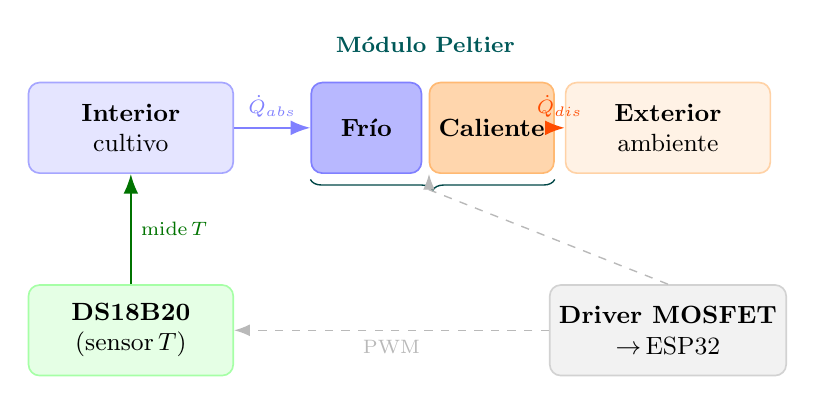
\begin{tikzpicture}[
    block/.style={draw, rounded corners=4pt, line width=0.6pt,
      minimum width=2.6cm, minimum height=1.15cm,
      align=center, font=\small},
    arr/.style={-{Latex[length=2.5mm]}, line width=0.7pt},
    darr/.style={-{Latex[length=2mm]}, dashed, line width=0.5pt, gray!55}
]
% --- Bloques principales ---
\node[block, fill=blue!10, draw=blue!35] (int)
      {\textbf{Interior}\\cultivo};
\node[block, fill=orange!10, draw=orange!35, right=4.2cm of int] (ext)
      {\textbf{Exterior}\\ambiente};

% --- M\'odulo Peltier (dos caras) ---
\node[block, fill=blue!28, draw=blue!50,
      minimum width=1.4cm, font=\small\bfseries]
      (frio) at ($(int.east)!0.40!(ext.west)$) {Fr\'io};
\node[block, fill=orange!32, draw=orange!55,
      minimum width=1.4cm, font=\small\bfseries,
      right=0.08cm of frio] (cal) {Caliente};

% --- Etiqueta Peltier ---
\node[above=0.25cm of frio, xshift=0.75cm,
      font=\footnotesize\bfseries, text=teal!70!black]
      {M\'odulo Peltier};
\draw[decorate, decoration={brace, amplitude=4pt, mirror},
      line width=0.5pt, teal!55!black]
      ([yshift=-2pt]frio.south west) -- ([yshift=-2pt]cal.south east);

% --- Flechas de flujo de calor ---
\draw[arr, blue!50] (int.east) -- (frio.west)
      node[midway, above, font=\scriptsize, text=blue!50] {$\dot{Q}_{abs}$};
\draw[arr, orange!60!red] (cal.east) -- (ext.west)
      node[midway, above, font=\scriptsize, text=orange!60!red] {$\dot{Q}_{dis}$};

% --- Sensor y driver ---
\node[block, fill=green!10, draw=green!35,
      below=1.4cm of int] (sens)
      {\textbf{DS18B20}\\(sensor\,$T$)};
\node[block, fill=gray!10, draw=gray!35,
      below=1.4cm of ext] (drv)
      {\textbf{Driver MOSFET}\\$\rightarrow$\,ESP32};

% --- Conexiones ---
\draw[arr, green!45!black] (sens) -- (int)
      node[midway, right, font=\scriptsize, text=green!45!black]
      {mide\,$T$};
\draw[darr] (drv.north) -- ($(frio.south)!0.5!(cal.south)+(0,-0.2)$)
      -- ($(frio.south)!0.5!(cal.south)$);
\draw[darr] (drv.west) -- (sens.east)
      node[midway, below, font=\scriptsize, text=gray!55] {PWM};
\end{tikzpicture}%
}
\caption{Corte esquem\'atico del montaje del m\'odulo Peltier en la pared
del reactor: cara fr\'ia hacia el cultivo, cara caliente disipada al
exterior, con realimentaci\'on desde el sensor interior hacia el driver.}
\label{fig:arquitectura}
\end{figure}

% =====================================================================
\section{Estrategia de Control}
% =====================================================================

Se propone un esquema de \textbf{control en cascada con supervisi\'on}, compuesto por:

\subsection{Supervisor de hist\'eresis}
Una m\'aquina de estados decide el estado $s \in \{0,1\}$ de la camisa
(cerrada/abierta). Para el entorno tropical de Santa Marta, la l\'ogica 
biol\'ogica (nictinastia) se \textbf{invierte} intencionalmente: la camisa se cierra 
de d\'ia para bloquear la irradiancia extrema (aislando el cultivo), y se 
abre de noche para permitir enfriamiento pasivo, aligerando la carga del Peltier:
\begin{equation}
s =
\begin{cases}
0 \ (\text{cerrar}) & \text{si hay irradiancia o } T_{ext} > T_{int} \\
1 \ (\text{abrir}) & \text{si es de noche y } T_{ext} \leq T_{int}
\end{cases}
\label{eq:supervisor}
\end{equation}

\subsection{Lazo PID y prealimentaci\'on}
El modelo t\'ermico del reactor considera la conmutaci\'on de la resistencia t\'ermica de la camisa. Cuando se requiere enfriamiento activo, un controlador PID ajusta la potencia del m\'odulo Peltier bas\'andose en el error de temperatura interior. 

Dado que la irradiancia solar es la perturbaci\'on dominante, se a\~nade un t\'ermino anticipativo (\textit{feedforward}) proporcional a esta irradiancia sobre la salida del PID. Esto permite al controlador reaccionar a la carga t\'ermica antes de que el error de temperatura se manifieste en el cultivo.

% =====================================================================
\section{Conclusiones}
% =====================================================================

El an\'alisis biomim\'etico de \textit{Espeletia occulta} subsp.
\textit{glossophylla} produjo seis mecanismos de regulaci\'on t\'ermica
transferibles a un dise\~no de ingenier\'ia, de los cuales el aislamiento
variable (nictinastia adaptada al tr\'opico) y la masa t\'ermica distribuida (m\'edula
capacitiva) se combinaron en un diferencial coherente: una camisa
aislante de apertura program\'atica junto con enfriamiento activo mediante
m\'odulo Peltier, coordinados por un control en cascada con
prealimentaci\'on. Los par\'ametros de cultivo de \textit{Chlorella
vulgaris} documentados en la literatura --particularmente el umbral de
estr\'es t\'ermico entre 30 y 35\,\textdegree C-- validan de forma
independiente el l\'imite cr\'itico ya establecido en los indicadores del
prototipo. El trabajo futuro inmediato consiste en la identificaci\'on
param\'etrica del modelo t\'ermico, la sinton\'ia del controlador PID y la
implementaci\'on f\'isica del prototipo para el Capstone Project I.

% =====================================================================
% BIBLIOGRAFIA
% =====================================================================
\begin{thebibliography}{00}

\bibitem{guiaaluna}
Semillero ProtopIA, ``ALUNA PBRs -- Fotobiorreactores Bioinspirados: Gu\'ia
Orientadora Integral e Ilustrada,'' Programa de Ingenier\'ia
Electr\'onica, Universidad del Magdalena, Capstone Project I, Control II,
2026-II. (Material interno del curso, no publicado.)

\bibitem{pmc12729280}
``Growth of \textit{Chlorella vulgaris} Under Atmospheric CO$_2$ in
Lab-Scale Photobioreactors: Effects of Aeration Rate and Growth Model
Comparison,'' \textit{PMC}, 2026. [Online]. Available:
\url{https://pmc.ncbi.nlm.nih.gov/articles/PMC12729280/}

\bibitem{researchgate348063343}
``Determination of Growth Conditions for \textit{Chlorella vulgaris},''
\textit{ResearchGate}, 2026. [Online]. Available:
\url{https://www.researchgate.net/publication/348063343}

\bibitem{christwardana2022}
A. Christwardana, ``Optimization of light intensity and color temperature
in the cultivation of \textit{Chlorella vulgaris} culture using the
Surface Response Method,'' \textit{J. Bioresources Environ. Sci.}, 2022.
[Online]. Available: \url{https://jbes.cbiore.id/index.php/jbes/article/view/14410}

\bibitem{sciencedirect2024phyto}
``Optimal growth conditions to enhance \textit{Chlorella vulgaris} biomass
production in indoor phyto tank and quality assessment of feed and
culture stock,'' \textit{ScienceDirect}, 2024. [Online]. Available:
\url{https://www.sciencedirect.com/science/article/pii/S2405844024079313}

\bibitem{wong2017}
Y.\,K. Wong, Y.\,H. Ho, K.\,C. Ho, \textit{et al.}, ``Growth medium
screening for \textit{Chlorella vulgaris} growth and lipid productions,''
\textit{J. Aquac. Mar. Biol.}, vol.~6, no.~1, pp.~203--209, 2017.

\bibitem{sciencedirect2026temp}
``Temperature effects on growth and biochemical composition of
\textit{Chlorella vulgaris} under heterotrophic cultivation,''
\textit{ScienceDirect}, 2026. [Online]. Available:
\url{https://www.sciencedirect.com/science/article/pii/S0981942826004171}

\bibitem{mdpi2854}
``Heat Stress Resistance in \textit{Chlorella vulgaris} Enhanced by
Hydrolyzed Whey Proteins,'' \textit{Agriculture (MDPI)}, vol.~14, no.~12,
art.~2854, 2024. [Online]. Available: \url{https://www.mdpi.com/2073-4395/14/12/2854}

\bibitem{plants2019}
``Effect of Light Intensity and Quality on Growth Rate and Composition of
\textit{Chlorella vulgaris},'' \textit{Plants (MDPI)}, vol.~9, no.~1,
art.~31, 2019. [Online]. Available: \url{https://www.mdpi.com/2223-7747/9/1/31} (PMCID: \url{https://pmc.ncbi.nlm.nih.gov/articles/PMC7020147/})

\bibitem{blueLED2023}
``The Effect of Optimum Photoperiod from Blue LED Light on Growth of
\textit{Chlorella Vulgaris} in Photobioreactor Tank,'' \textit{ResearchGate},
2023. [Online]. Available:
\url{https://www.researchgate.net/publication/372287904}

\bibitem{blueLED2013}
``Intensity of blue LED light: A potential stimulus for biomass and lipid
content in fresh water microalgae \textit{Chlorella vulgaris},''
\textit{ScienceDirect}, 2013. [Online]. Available:
\url{https://www.sciencedirect.com/science/article/abs/pii/S096085241301420X}

\bibitem{sciencedirect2018photon}
``Growth rates and photon efficiency of \textit{Chlorella vulgaris} in
relation to photon absorption rates under different LED-types,''
\textit{ScienceDirect}, 2018. [Online]. Available:
\url{https://www.sciencedirect.com/science/article/abs/pii/S2211926417305246}

\bibitem{scenedesmus2023}
``Evaluation of Growth and Production of High-Value-Added Metabolites in
\textit{Scenedesmus quadricauda} and \textit{Chlorella vulgaris} Grown on
Crude Glycerol under Heterotrophic and Mixotrophic Conditions Using
Monochromatic Light-Emitting Diodes (LEDs),'' \textit{PMC}, 2023. [Online].
Available: \url{https://www.ncbi.nlm.nih.gov/pmc/articles/PMC10453295/}

\end{thebibliography}

\end{document}